\section{Spørsmål; Runde 5}
Jeg har prøv å kjøre simuleringer med dataen jeg har for øyeblikket. Resultatene er vist 
lengre nede og ser ikke helt fornuftige ut. Dette dokumentet inneholder derfor
en kjapp gjennomgang av hva jeg har gjort, for å eksludere at jeg ikke har missforstått noe.
All data som er brukt i denne gjennomkjøringen er fra de artiklene du sendte meg tidligere
(til jorgevag@stud.ntnu.no).

\subsection{Data hentet ut fra artiklene}
I figurene 
\ref{fig1E},
\ref{fig2E},
\ref{fig3E},
er grafene funnet i artiklene vist i mot den dataen som faktisk ble hentet ut. I Figur
\ref{fig1E}
er det blandt annet mest overlapp og størst sjanse for feil. Kan også hende at
grafene i den uthentede dataen krysser hverandre feil i de mest overlappede regionene.
\newpage
%
\begin{figure}[h!] 
\centering 
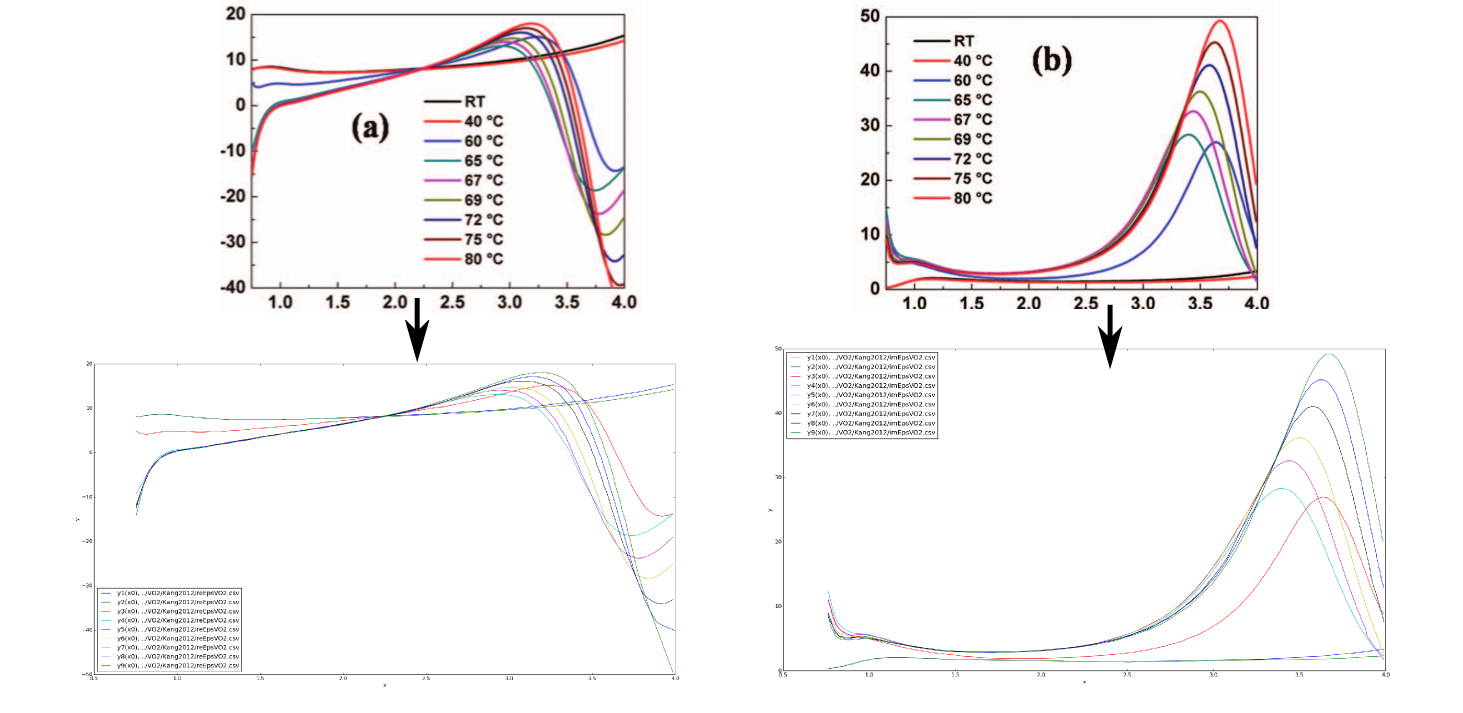
\includegraphics[width=1.0\textwidth]{Figures/KangExtraction.png} 
\caption{Extraction of data from Kang.}
\label{fig1E}
\end{figure}
%
\begin{figure}[h!] 
\centering 
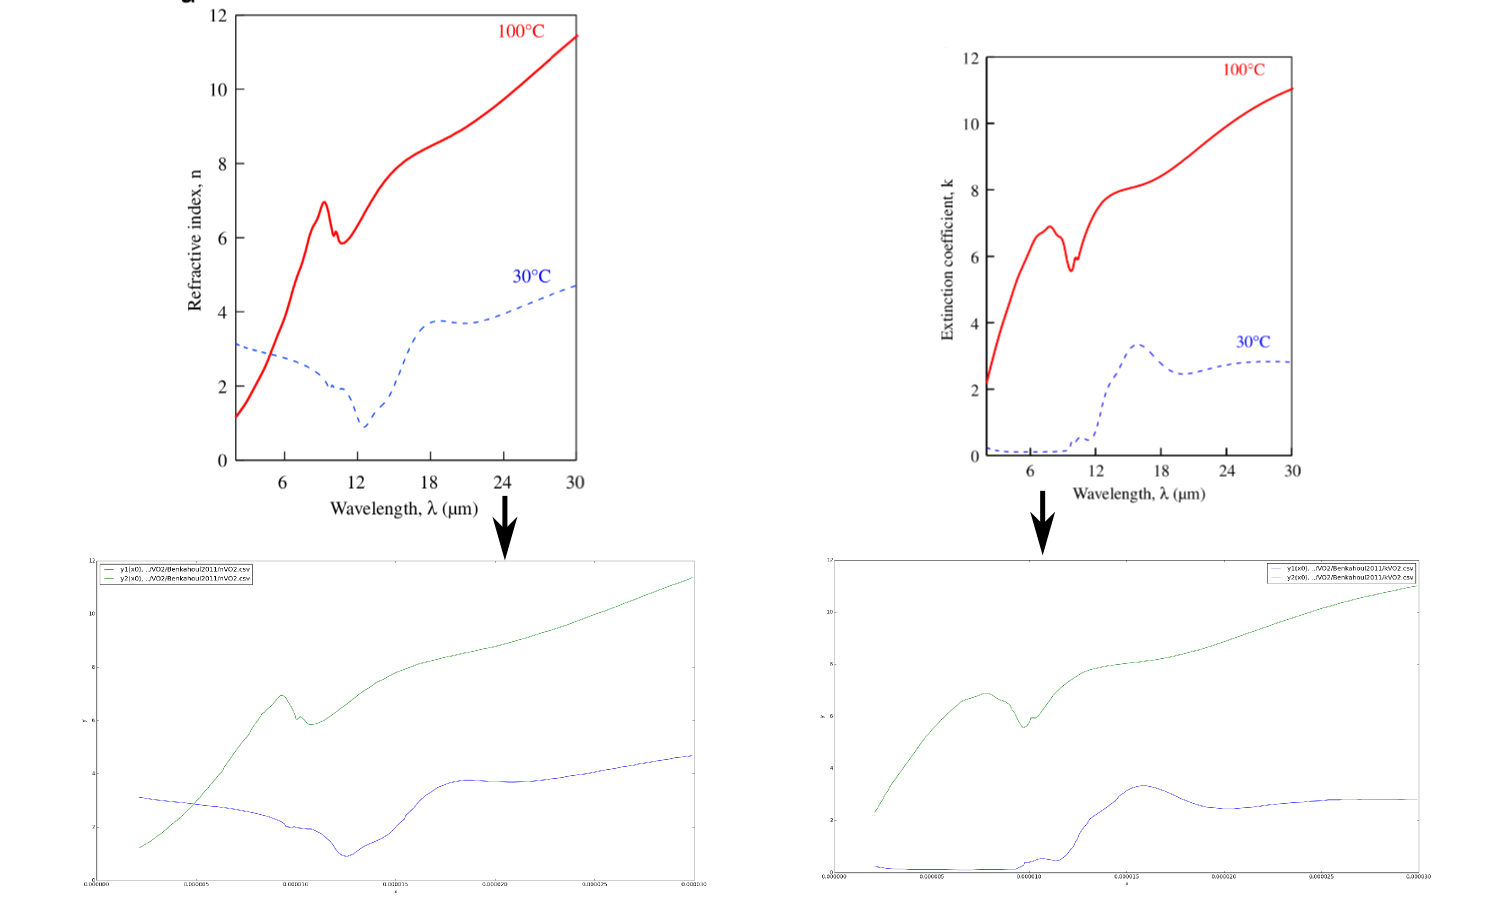
\includegraphics[width=1.0\textwidth]{Figures/BenkahoulExtraction.png} 
\caption{Extraction of data from Benkahoul.}
\label{fig2E}
\end{figure}
%
\begin{figure}[h!] 
\centering 
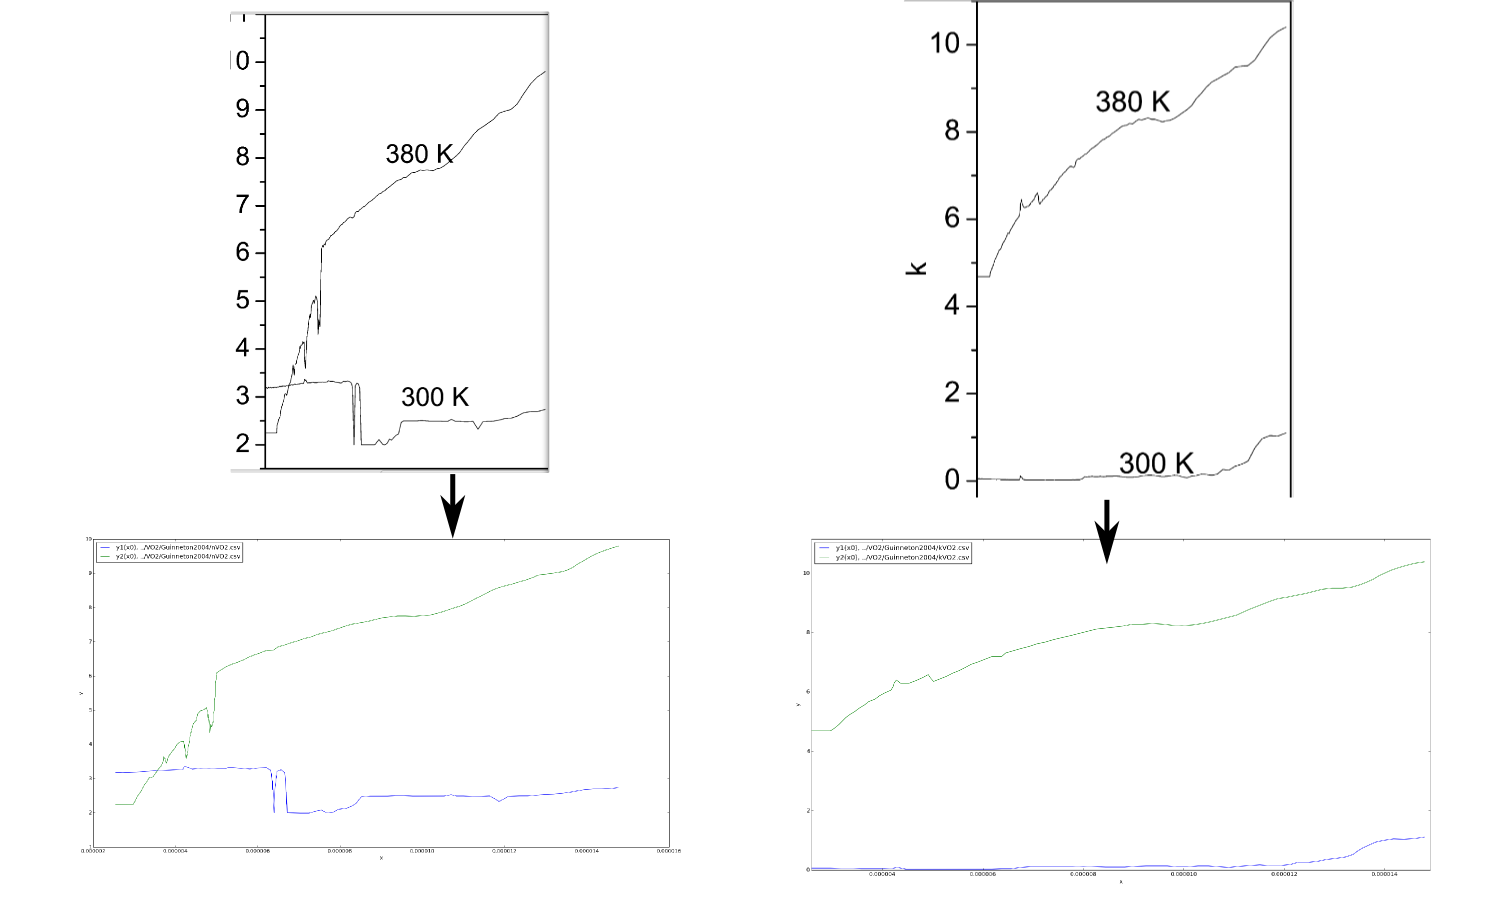
\includegraphics[width=1.0\textwidth]{Figures/GuinnetonExtraction.png} 
\caption{Extraction of data from Guinneton}
\label{fig3E}
\end{figure}
%


\newpage
\subsection{Konvertering av data}
For å konvertere dataen til ekvidistansert n,k-data, brukte jeg samme 
metode som det interpoleringsprogrammet du hjap meg med tidligere. 
Uavhengig om hva enhetene på dataen var, valgte jeg å intrapolere til ekvidistansert
data før jeg konverterte til kompleks brytningsindeks. 
Jeg brukte følgende kode for å konvertere den intrapolerte dataen, som 
her er gitt ved \textbf{re}, \textbf{im} (som kan være permittivitet $\varepsilon$ eller 
brytningsindeks$\hat{n})$:
\begin{lstlisting}[style=FormattedNumber, language=python]
# If the input data is the permittivity/dielectric function, 
# we have to convert to the refractive indicies n,k:
if( isPermittivity ): # data is permittivity
    import scipy.constants
    epsilon0 = scipy.constants.epsilon_0
    # convert from permittivity to refractive index n and absorbtion coeff k:
    absEpsilon = numpy.sqrt( re**2 + im**2)
    n = numpy.sqrt( (absEpsilon + re)/2.0*epsilon0 )
    k = numpy.sqrt( (absEpsilon - re)/2.0*epsilon0 )
else: # the real data should be n, and the imaginary data should be k:
    n = re
    k = im


# convert the x-values to the correct output units: unit=1->x[eV] or unit=2->x[micrometers]
if( unit == 1 ): # eV
    pass # Do nothing
elif(unit == 2): # micrometers
    pass # Do nothing
elif(unit == 3): # nm
    x_min = x_min*(10**(-3))
    x_max = x_max*(10**(-3))
    unit = 2
elif(unit == 4): # m
    x_min = x_min*(10**(6))
    x_max = x_max*(10**(6))
    unit = 2

#write to file
firstLine = str(unit)+'\t'+str(x_min)+'\t'+str(x_max)+'\t'+str(dataPoints)  
numpy.savetxt(ofile, numpy.column_stack((n,k)), delimiter='\t', header=firstLine, comments='')
\end{lstlisting}
For å regne om til n og k, antar jeg at dataen er gitt som $\hat\varepsilon = \hat\varepsilon_r \varepsilon_0$
og bruker:
\begin{align}
   n      &= \sqrt{ \frac{|\hat{\varepsilon}_r| + \varepsilon_r}{2}} 
           = \sqrt{ \frac{|\hat{\varepsilon}| + \varepsilon}{2\varepsilon_0}}\\
   \kappa &= \sqrt{ \frac{|\hat{\varepsilon}_r| - \varepsilon_r}{2}} 
           = \sqrt{ \frac{|\hat{\varepsilon}| - \varepsilon}{2\varepsilon_0}}.
\end{align}

Før jeg leser inn dataen til \textsc{GranFilm}, endrer jeg på 'Energy\_Range' i '.sif'-filen ved å 
lese første linje fra '.nk'-filen. Om verdiene er gitt i $\mu$m (unit=2), konverterer 
jeg med følgende kode (før det skrives inn i '.sif'-filen):
\begin{lstlisting}[style=FormattedNumber, language=python]
# Get 'unit' and energy interval [x1,x2]:
nkfileInfo = nkfileLine1.split()
unit = int(nkfileInfo[0])
x1 = float(nkfileInfo[1])
x2 = float(nkfileInfo[2])

# Check unit:
if( unit == 1 ): # eV
    Emin = x1
    Emax = x2

if( unit == 2 ): # micrometer (wavelength)
    #then convert to eV:
    import scipy.constants as sc
    h = sc.h/sc.e # (planck's constant[J s])/(elementary charge) = planck[eV s]
    c = sc.c # speed of light

    Emin = h*c/( x2*(10**(-6)) )
    Emax = h*c/( x1*(10**(-6)) )
    #ref: http://www.pveducation.org/pvcdrom/properties-of-sunlight/energy-of-photon
\end{lstlisting}
Deretter kjøres \textsc{GranFilm} med'.sif'-filen som input, som igjen kaller tilhørende '.nk'-fil.



\subsection{Test-Simulering}
Dataen nevnt ovenfor ble konvertert til kompleks brytningsindeks og matet inn i GranFilm.
Når all dataen ble simulert (Fig.\ref{figAllD}), så det ut til at den delte seg inn 
i 3 ''regioner'', of jeg frykter dette skyldes ulikheter fra de 3 artiklene.
%
\begin{figure}[h!] 
\centering 
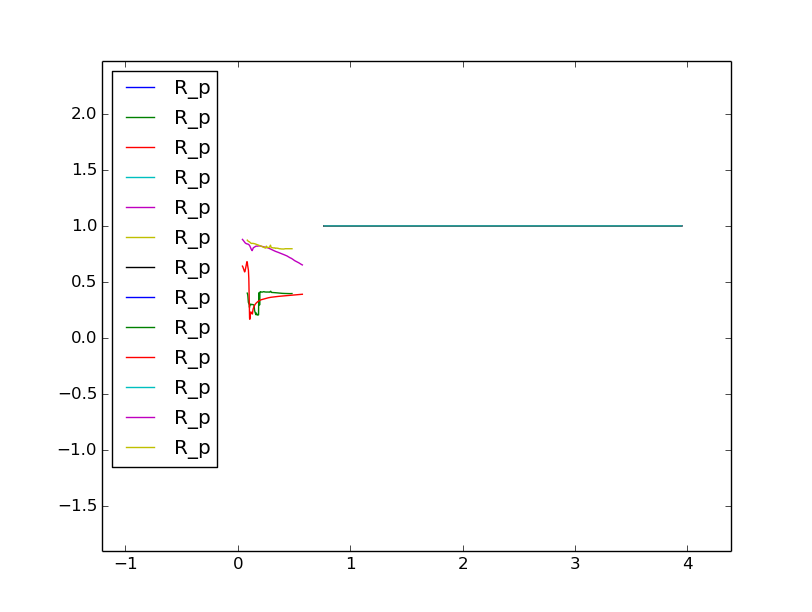
\includegraphics[width=0.5\textwidth]{Figures/vo2RpAll.png} 
\caption{Plot of $R_p = \sqrt{Re(r_p)^2 + Im(r_p)^2}$ for all extracted temperature-data.
Looks like it has formed three different regions shifted from one another.}
\label{figAllD}
\end{figure}
%
%
\begin{figure}[h!] 
\centering 
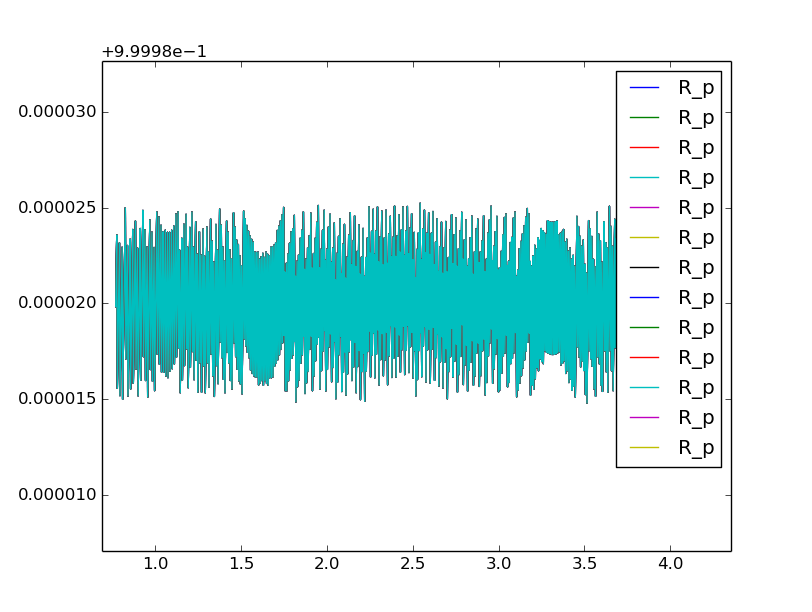
\includegraphics[width=0.5\textwidth]{Figures/kangDataSimulated.png} 
\caption{If I zoom in on the flat part (in $R_p$-plot on previous figure), it looks really messy.}
\label{figAllD1}
\end{figure}
%
En nærmere titt på den flate delen til høyre i Fig.\ref{figAllD}, er vist 
i Fig.\ref{figAllD1}, og jeg får på følelsen av at noe er veldig feil.
Til venstre, Fig. \ref{figAllD2}, ser derimot bedre ut, men vet ikke helt
om resultatet virker fornuftig eller ikke.
%
\begin{figure}[h!] 
\centering 
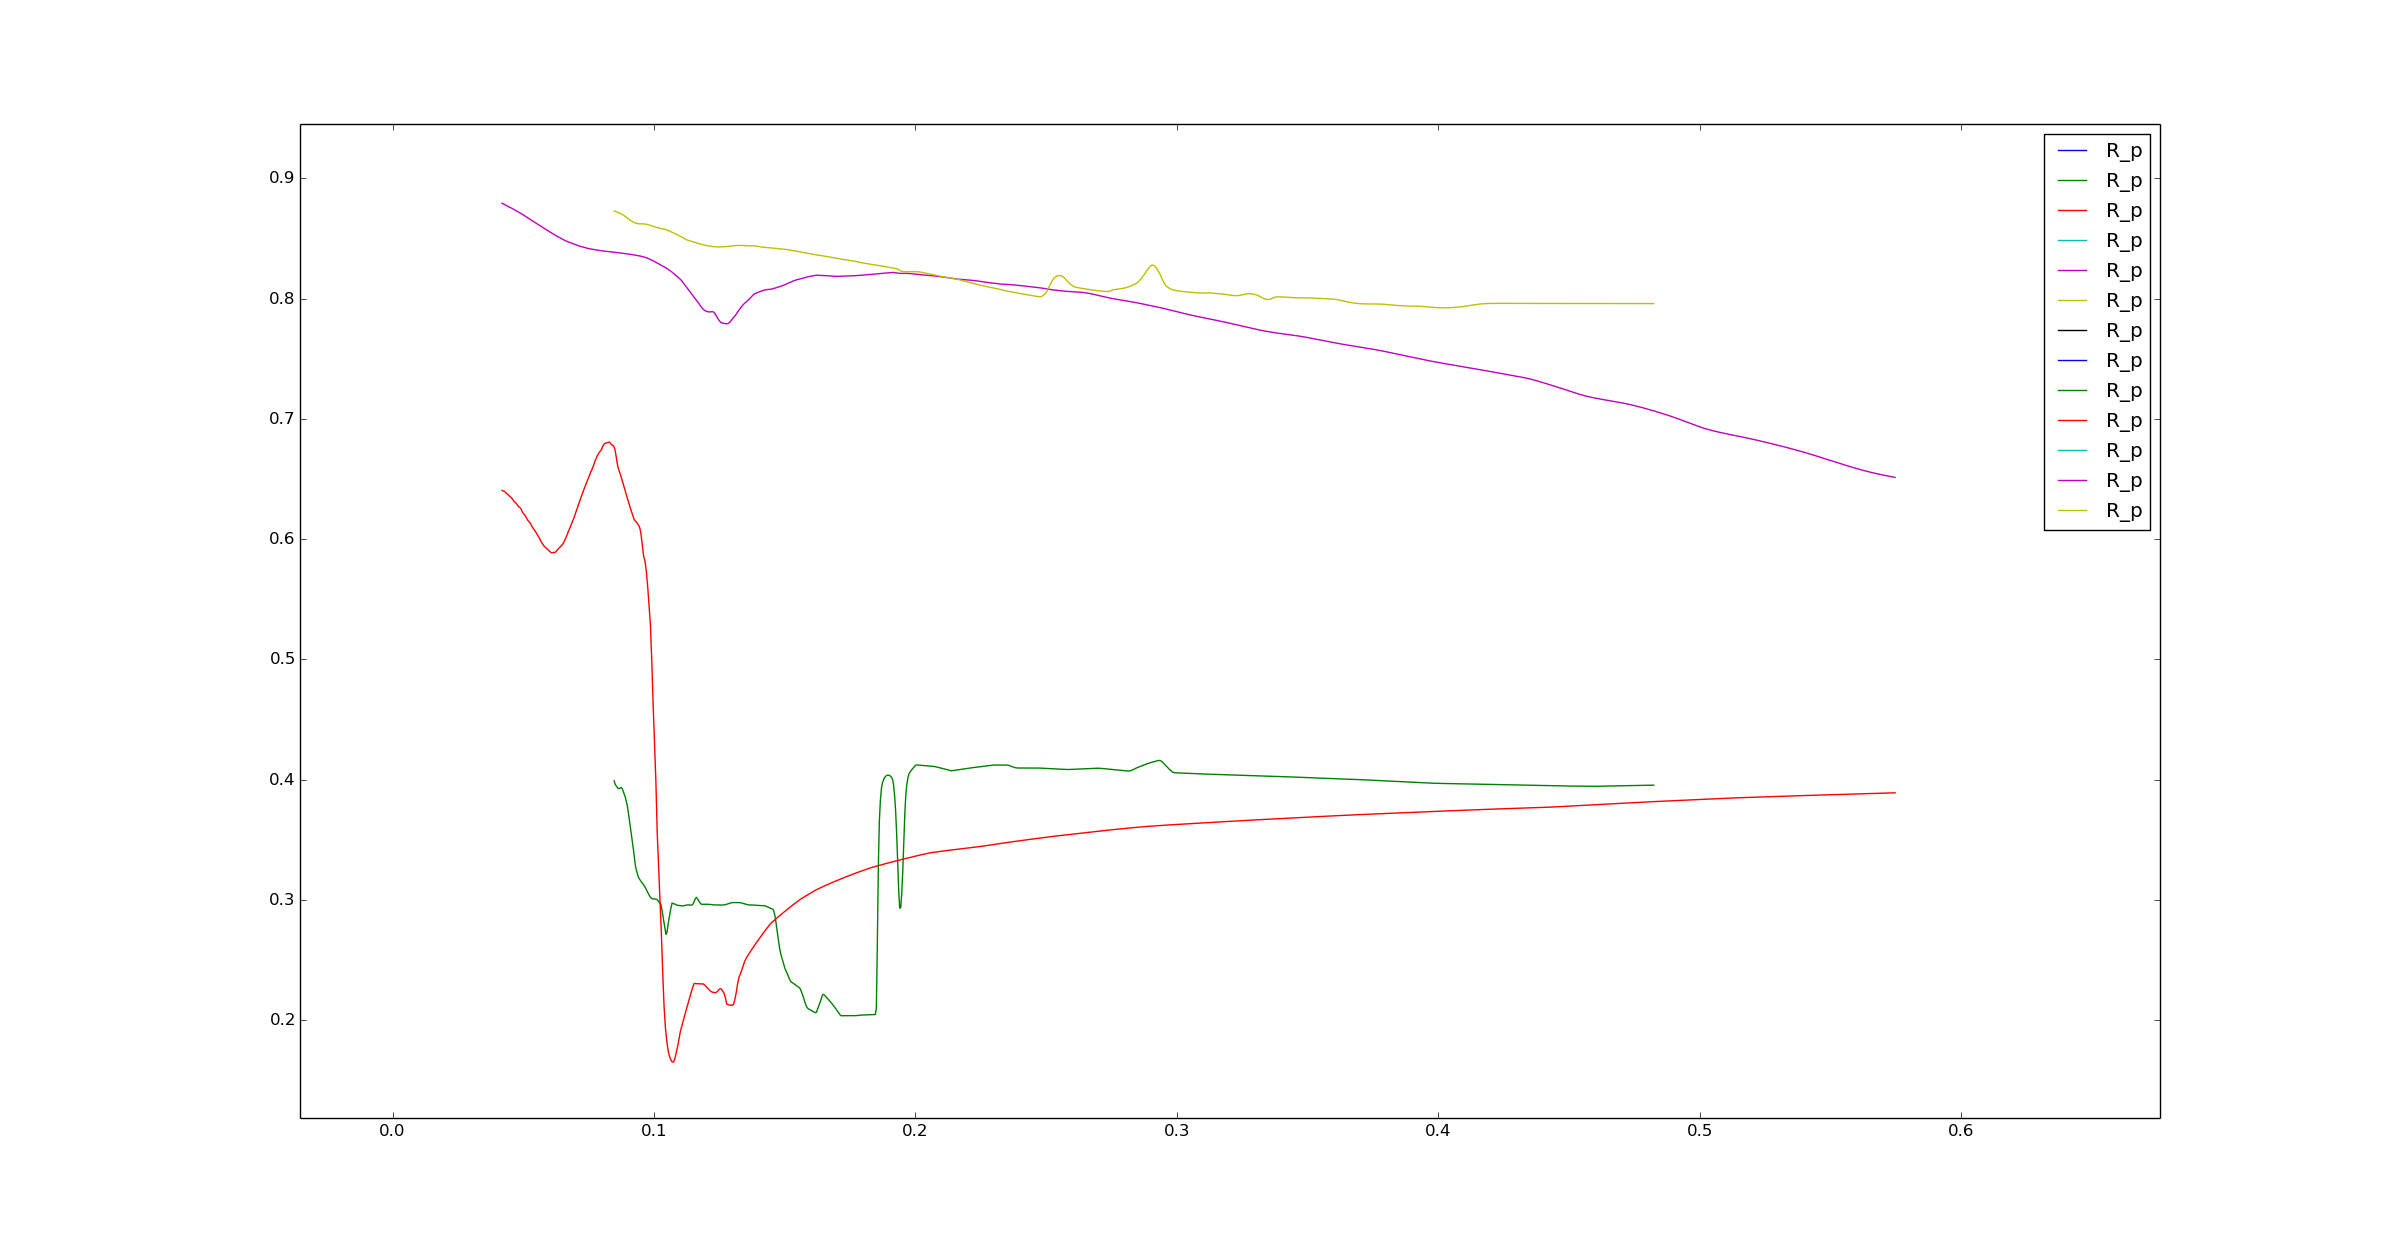
\includegraphics[width=0.5\textwidth]{Figures/niceData.png} 
\caption{The other data in the $R_p$-plot.}
\label{figAllD2}
\end{figure}
%


Sist ble det gjort en simulering for $T = 300$K og $T = 380$K med dataen fra Guinnetion.
Refleksjon og Transmisjon for p-polarizert lys er gitt i Fig.\ref{fig1D} og Fig.\ref{fig2D}.
%
\begin{figure}[h!] 
\centering 
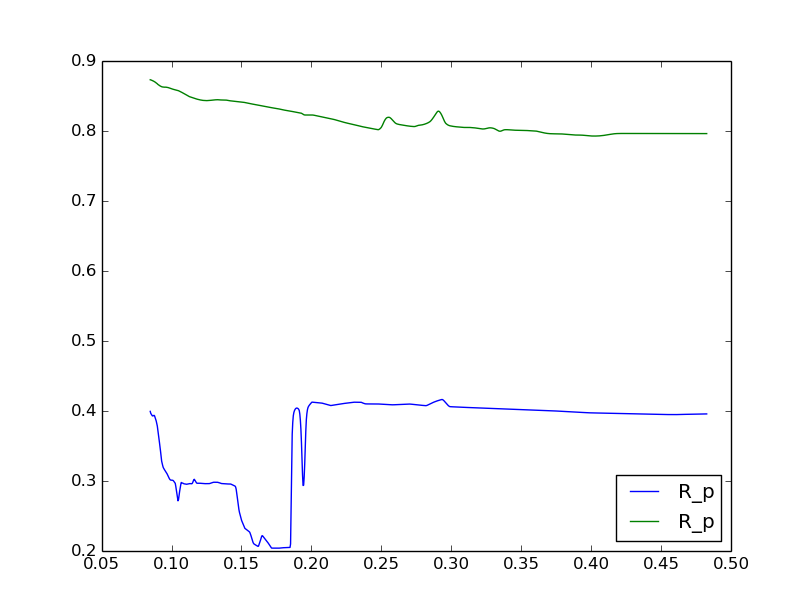
\includegraphics[width=0.5\textwidth]{Figures/vo2Rp_blue300K_green380K.png} 
\caption{ $R_p$ from Guinneton. The blue line is for $T = 300$K; The green line is for $T=380$K.}
\label{fig1D}
\end{figure}
%
%
\begin{figure}[h!] 
\centering 
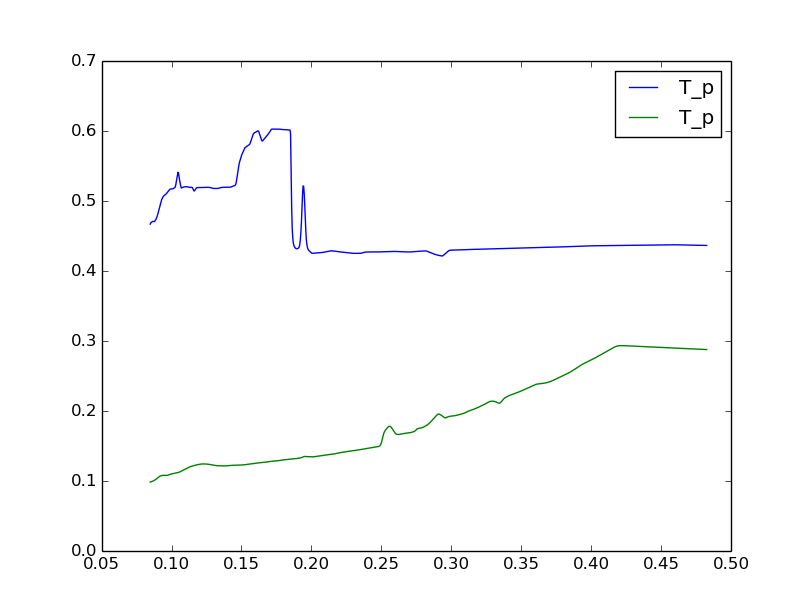
\includegraphics[width=0.5\textwidth]{Figures/vo2Tp_blue300K_green380K.png} 
\caption{ $T_p$ from Guinneton. The blue line is for $T = 300$K; The green line is for $T=380$K.}
\label{fig2D}
\end{figure}
%
\newpage
Jeg er på dette tidspunktet veldig usikker på hvordan jeg finner ut om resultatene er fornuftig eller
feil. Med tanke på hvordan Fig.\ref{figAllD} og Fig.\ref{figAllD1} ser ut, vil jeg uansett anta at 
noe er fryktelig feil. 
\textbf{Er du enig i at dette ser feil ut og har du noen forslag til hva som kan være feil?}
